%%%%%%%%%%%%%%%%%%%%%%%%%%%%%%%%%%%%%%%%%%  不使用 authblk 包制作标题  %%%%%%%%%%%%%%%%%%%%%%%%%%%%%%%%%%%%%%%%%%%%%%
%-------------------------------PPT Title-------------------------------------
\title{05-赝势理论}
%-----------------------------------------------------------------------------

%----------------------------Author & Date------------------------------------
%\author[\textrm{Jun\_Jiang}]{姜\;\;骏\inst{}} %[]{} (optional, use only with lots of authors)
%% - Give the names in the same order as the appear in the paper.
%% - Use the \inst{?} command only if the authors have different
%%   affiliation.
\institute[BCC]{\inst{}%
%\institute[Gain~Strong]{\inst{}%
\vskip -20pt 北京市计算中心}
%\vskip -20pt {\large 格致斯创~科技}}
\date[\today] % (optional, should be abbreviation of conference name)
{%	{\fontsize{6.2pt}{4.2pt}\selectfont{\textcolor{blue}{E-mail:~}\url{jiangjun@bcc.ac.cn}}}
\vskip 45 pt {\fontsize{8.2pt}{6.2pt}\selectfont{%清华大学\;\;物理系% 报告地点
	\vskip 5 pt \textrm{2022.07.22}}}
}

%% - Either use conference name or its abbreviation
%% - Not really information to the audience, more for people (including
%%   yourself) who are reading the slides onlin%%   yourself) who are reading the slides onlin%%   yourself) who are reading the slides onlineee
%%%%%%%%%%%%%%%%%%%%%%%%%%%%%%%%%%%%%%%%%%%%%%%%%%%%%%%%%%%%%%%%%%%%%%%%%%%%%%%%%%%%%%%%%%%%%%%%%%%%%%%%%%%%%%%%%%%%%

\subject{}
% This is only inserted into the PDF information catalog. Can be left
% out.
%\maketitle
\frame
{
%	\frametitle{\fontsize{9.5pt}{5.2pt}\selectfont{\textcolor{orange}{“高通量并发式材料计算算法与软件”年度检查}}}
\titlepage
}
%-----------------------------------------------------------------------------

%------------------------------------------------------------------------------列出全文 outline ---------------------------------------------------------------------------------
%\section*{}
%\frame[allowframebreaks]
%{
%  \frametitle{Outline}
%%  \frametitle{\textcolor{mycolor}{\secname}}
%  \tableofcontents%[current,currentsection,currentsubsection]
%}
%%在每个section之前列出全部Outline
%%类似的在每个subsection之前列出全部Outline是\AtBeginSubsection[]
%\AtBeginSection[]
%{
%  \frame<handout:0>%[allowframebreaks]
%  {
%    \frametitle{Outline}
%%全部Outline中,本部分加亮
%    \tableofcontents[current,currentsection]
%  }
%}

%-----------------------------------------------PPT main Body------------------------------------------------------------------------------------
\small
\section{固体能带理论}
\frame
{
%\frametitle{The methods on band structure calculation}
\frametitle{固体能带计算方法}
%\vskip 10pt
%\textrm{The mainly difference of all these methods below: the basis sets and the construction of the potential}
\vskip 10pt
常用的计算方法
\begin{itemize}%[+-| alert@+>]
%\begin{enumerate}%[+-| alert@+>]
\setlength{\itemsep}{12pt}
%  \item \textrm{Plane wave and the pseudo-potential}
	\item	平面波方法
	\item	正交平面波\textrm{(The orthogonalized plane wave, OPW)}和赝势\textrm{(Pseudo-potential, PP)}方法\upcite{Singh,PRB41-7892_1990,JPCM6-8245_1994}
	\item	缀加平面波\textrm{(Augmented plane wave, APW)}方法
	\item	\textrm{MT}轨道\textrm{(Muffin-tin orbitals, MTO)}方法
	\item	投影子缀加波\textrm{(Projector Augmented Wave, PAW)}方法\upcite{PRB50-17953_1994,PRB59-1758_1999}
\end{itemize}
\vskip 5pt 各种方法的\textcolor{red}{主要区别}:~\textcolor{blue}{势函数的处理}与\textcolor{blue}{所选基函数类型}不同
}

\frame                               %
{
	\frametitle{\textrm{Kohn-Sham}方程}
\begin{figure}[h!]
\centering
\vspace*{-0.21in}
\hspace*{-0.1in}
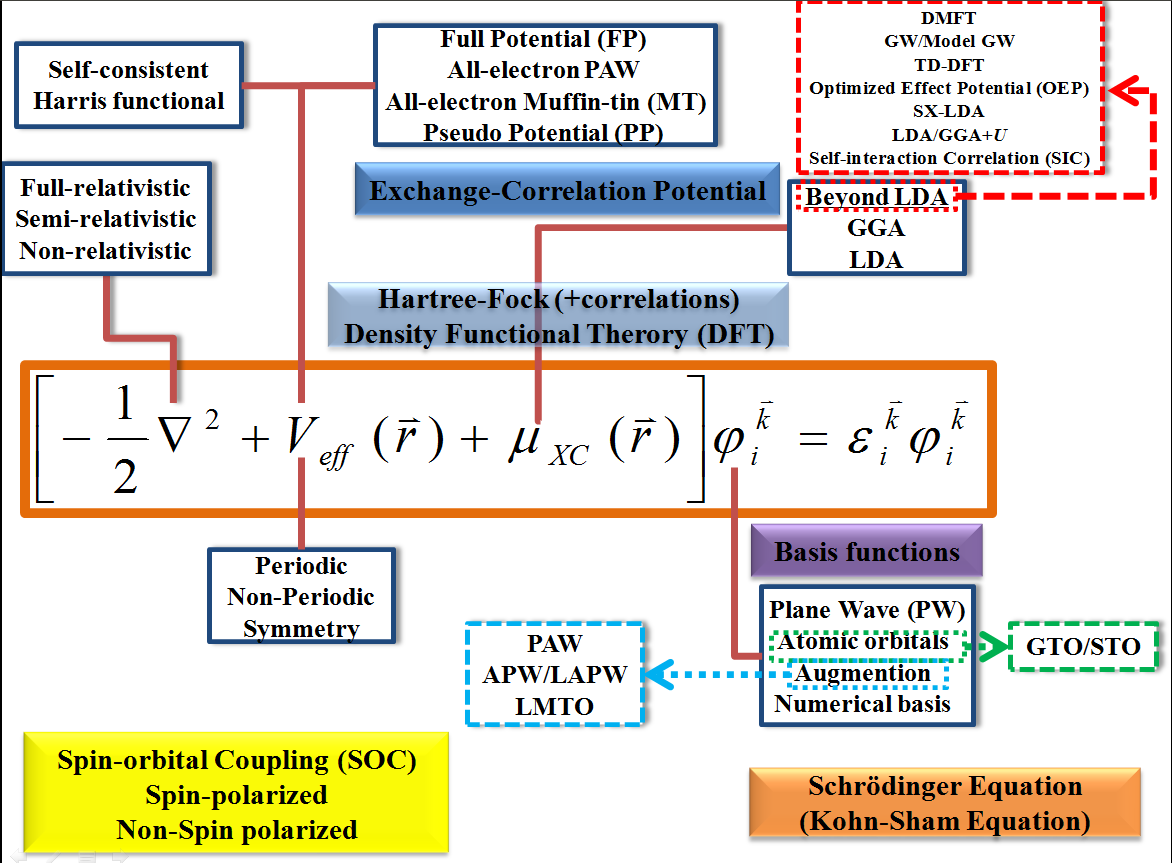
\includegraphics[height=2.7in,width=4.0in,viewport=2 5 1162 880,clip]{Figures/DFT.png}
\caption{\tiny \textrm{The Analysis of Kohn-Sham equation.}}%(与文献\cite{EPJB33-47_2003}图1对比)
\label{DFT}
\end{figure}
}

\frame
{
	\frametitle{\textrm{DFT-SCF}}
\begin{figure}[h!]
\centering
\vspace*{-0.25in}
\hspace*{-0.80in}
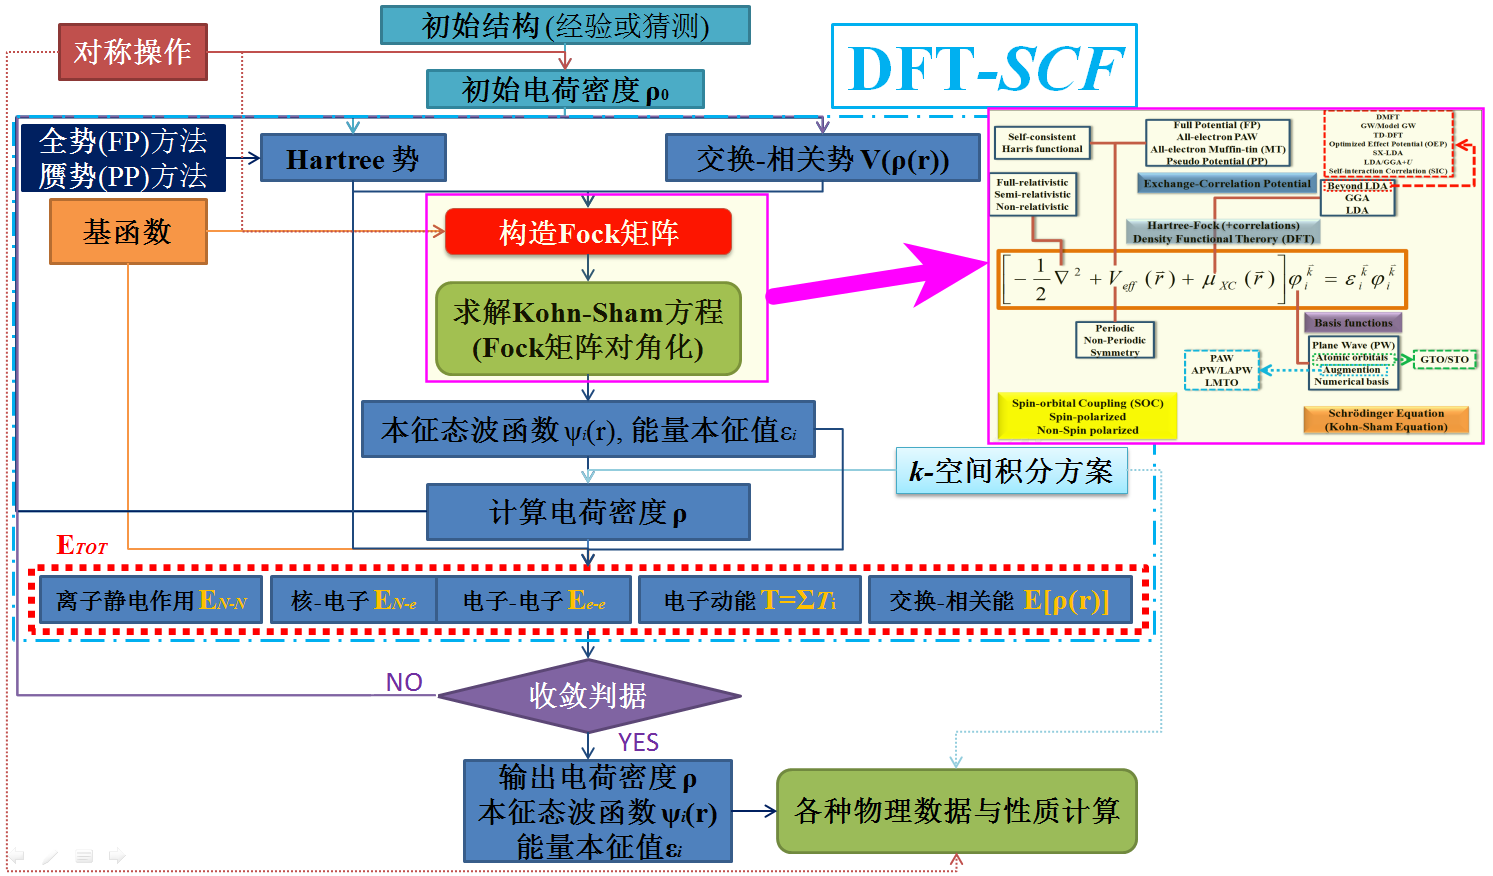
\includegraphics[height=2.80in,width=4.95in,viewport=5 3 1490 870,clip]{Figures/DFT-SCF_2.png}
%\caption{\tiny \textrm{Pseudopotential for metallic sodium, based on the empty core model and screened by the Thomas-Fermi dielectric function.}}%(与文献\cite{EPJB33-47_2003}图1对比)
\label{DFT-SCF-2}
\end{figure}
}

\section{赝势理论}       %Bookmark
%\section{Induction on DFT and solid-state physics}       %Bookmark
\subsection{平面波与赝势}       %Bookmark
\frame
{
	\frametitle{球形势对平面波的散射与相移}
\begin{figure}[h!]
\centering
\vspace*{-0.26in}
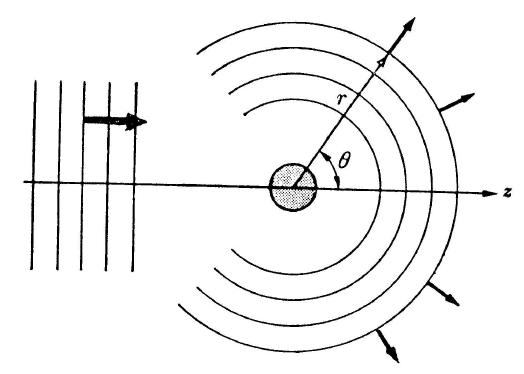
\includegraphics[height=0.90in,width=1.24in,viewport=0 0 400 300,clip]{Figures/Pseudo-scatter.jpg}
\caption{\fontsize{5.5pt}{4.2pt}\selectfont{\textrm{Schematic illustration of scattering of a plane wave by a spherical potential.}}}%(与文献\cite{EPJB33-47_2003}图1对比)
\label{Pseudo-scatter}
\end{figure}
\vspace*{-0.1in}
\fontsize{7.5pt}{6.2pt}\selectfont{
入射平面波
$$\mathrm{e}^{\mathrm{i}\vec q\cdot\vec r}=4\pi\sum_{lm}\mathrm{i}^lj_l(\vec q\cdot\vec r)Y_{lm}^{\ast}(\hat{\vec q})Y_{lm}(\hat{\vec r})=\sum_{l}(2l+1)\mathrm{i}^lj_l(qr)P_{l}(\cos\theta)$$
%$$\mathrm{e}^{\mathrm{i}\vec q\cdot\vec r}=\mathrm{e}^{\mathrm{i}qr\cos(\theta)}=\sum_{l}(2l+1)\mathrm{i}^lj_l(qr)P_{l}[\cos(\theta)]$$
经散射后出射,波函数变为
$$\Psi_l^{>}(\varepsilon,r)=C_l\bigg[j_l(\kappa r)-\tan\eta_l(\varepsilon)n_l(\kappa r)\bigg]\quad\text{其中}\kappa^2=\varepsilon$$
根据散射理论,能量为$\varepsilon$的电子经单个势阱散射偏转$\theta$后,波函数的振幅可以表示为
	\begin{displaymath}
		t(\theta)=\dfrac{4\pi}{\kappa}\sum_l(2l+1)[\mathrm{exp}(2\mathrm{i}\eta_l(\varepsilon))-1]P_l(\cos\theta)
	\end{displaymath}
%$$t(\theta)=\dfrac{4\pi}{\sqrt\varepsilon}\sum_l(2l+1)\bigg[\mathrm{e}^{2\mathrm{i}\eta_l(\varepsilon)}-1\bigg]P_l(\cos\theta)$$
%$$\eta_l(\varepsilon)=p_l\pi+\delta_l(\varepsilon)$$
}
}

\frame
{
	\frametitle{散射相移与赝势}
\begin{figure}[h!]
\centering
\vspace*{-0.25in}
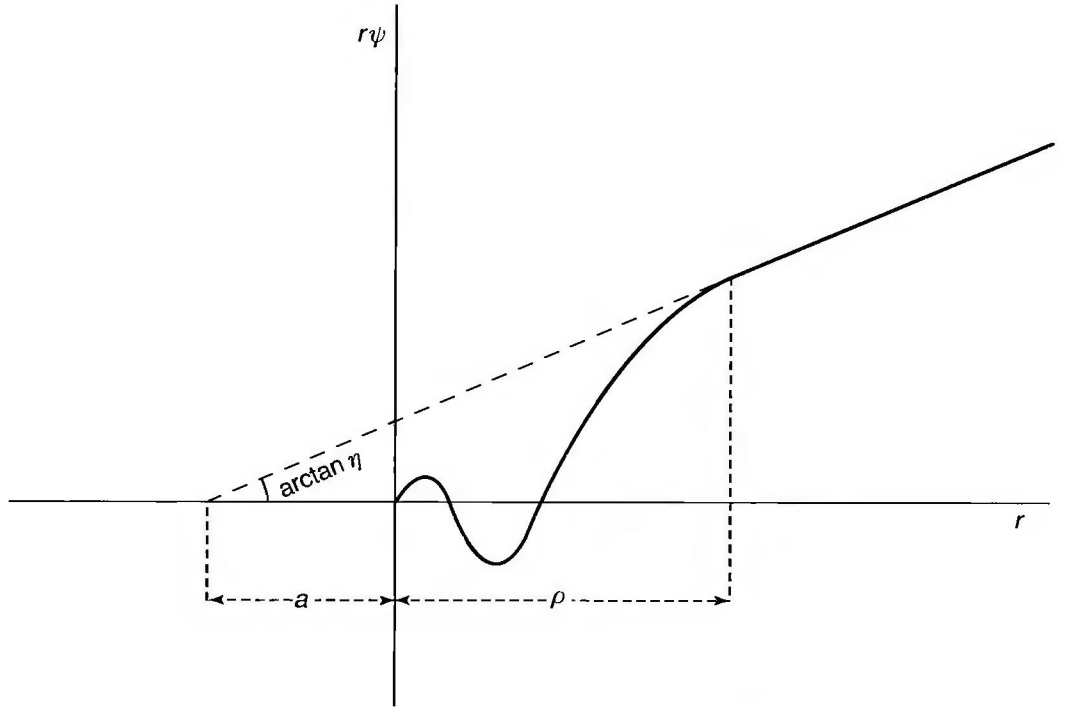
\includegraphics[height=1.20in,width=1.77in,viewport=0 0 1150 750,clip]{Figures/Pseudo-scatter-2.png}
\caption{\fontsize{4.5pt}{3.2pt}\selectfont{\textrm{Radial wave-function $\phi=r\psi$ for low-energy scattering as illustrated in a figure from the 1934 and 1935 papers of Fermi and coworkers for low-energy electron scattering from atoms and neutron scattering from nuclei. The node in the wave-function near the origin show that the potential is attractive and strong enough to have bound states. The cross-section for scattering from the localized potential is determined by the phase shift and is the same for weaker pseudo-potential with the same phase shift modulo $2\pi$.}}}%(与文献\cite{EPJB33-47_2003}图1对比)
\label{Pseudo-scatter-2}
\end{figure}
\fontsize{7.5pt}{6.2pt}\selectfont{
对于球形势散射,相移可由径向波函数计算
$$\tan\eta_l(\varepsilon)=\dfrac{R\frac{\mathrm{d}}{\mathrm{d}r}j_l(\kappa r)|_R-D_l(\varepsilon)j_l(\kappa R)}{R\frac{\mathrm{d}}{\mathrm{d}r}n_l(\kappa r)|_R-D_l(\varepsilon)n_l(\kappa R)}$$
$$\mbox{其中~}D_l(\varepsilon,r)\equiv r\psi_l^{\prime}(r)/\psi_l(r)=r\dfrac{\mathrm{d}}{\mathrm{d}r}\ln\psi_l(r)$$
同时相移与波函数节点的关系为:$$\eta_l(\varepsilon)=p_l\pi+\delta(\varepsilon)$$}
}

\frame
{
%\frametitle{The methods on band structure calculation}
	\frametitle{由\textrm{OPW~}到赝势}
%\vskip 10pt
%\textrm{The mainly difference of all these methods below: the basis sets and the construction of the potential}
\begin{itemize}
\setlength{\itemsep}{5pt}
	\item 完全平面波基组:~少数平面波就可以很好地描述波函数在原子间的行为,近核波函数则需要大量平面波展开。%因此完全平面波基组虽然方便,但求体系本征态对角化的矩阵非常巨大,计算变得异常耗时。
	\item 正交平面波(\textrm{Orthogonalized plane wave, OPW})方法,价电子用与芯层波函数正交的平面波展开
		\begin{displaymath}
			\phi_{OPW}^{\vec k+\vec G}(\vec r)=\phi_{PW}^{\vec k+\vec G}(\vec r)-\sum_c\langle\varphi_c|\phi_{PW}^{\vec k+\vec G}\rangle\varphi_c(\vec r)
		\end{displaymath}
		代入\textrm{Schr\"odinger}方程
		$$\hat H|\phi_{PW}^{\vec k+\vec G}\rangle-\sum_c\langle\varphi_c|\phi_{PW}^{\vec k+\vec G}\rangle\hat H|\varphi_c\rangle=\varepsilon|\phi_{PW}^{\vec k+\vec G}\rangle-\varepsilon\sum_c\langle\varphi_c|\phi_{PW}^{\vec k+\vec G}\rangle|\varphi_c\rangle$$
		可有$$\hat H|\phi_{PW}^{\vec k+\vec G}\rangle+\textcolor{blue}{V^R}|\phi_{PW}^{\vec k+\vec G}\rangle=\textcolor{blue}{\varepsilon}|\phi_{PW}^{\vec k+\vec G}\rangle$$
%		这里排斥势是$$V^R(\vec r,\vec r^{\prime})=\sum_c(\varepsilon-\varepsilon_c)|\varphi_c(\vec r^{\prime})\rangle\langle\varphi_c(\vec r)|$$
\end{itemize}
}

\frame
{
	\frametitle{由\textrm{OPW~}到赝势}
	\textrm{Phillips-Kleinman}指出赝势($V^{e\!f\!f}$)-赝波函数(可用$\phi_{PW}^{\vec k+\vec G}$展开)满足\textrm{Schr\"odinger}方程\upcite{PR116-287_1959}
	$$\bigg(-\dfrac12\nabla^2+\textcolor{red}{V^{e\!f\!f}}\bigg)|\phi_{PW}^{\vec k+\vec G}\rangle=\textcolor{blue}{\varepsilon}|\phi_{PW}^{\vec k+\vec G}\rangle$$
	其中$\textcolor{red}{V^{e\!f\!f}}=V(\vec r)+\textcolor{blue}{V^R}$
	\begin{itemize}
		\item 赝势-赝波函数的本征值$\varepsilon$与真实体系的能量本征值等价
		\item 赝势$V^{e\!f\!f}$比$V(\vec r)$平滑得多,并且$V^R$是非局域的排斥势
			\begin{displaymath}
				\begin{aligned}
					V^Rf(\vec r)=&\sum_c(\varepsilon-\varepsilon_c)\varphi_c(\vec r)\int\varphi_c^{\ast}(\vec r^{\prime})f(\vec r^{\prime})\mathrm{d}\vec r^{\prime} \\
					=&\int V^R(\vec r,\vec r^{\prime})f(\vec r^{\prime})\mathrm{d}\vec r^{\prime}
				\end{aligned}
			\end{displaymath}
			这里$$V^R(\vec r,\vec r^{\prime})=\sum_c(\varepsilon-\varepsilon_c)|\varphi_c(\vec r^{\prime})\rangle\langle\varphi_c(\vec r)|$$
	\end{itemize}
}

\frame
{
\frametitle{赝势方法}
赝势(\textrm{Pseudo Potential, PP})方法是在正交平面波的基础上发展起来的,构造出平缓的势函数代替核的强吸引作用和芯层电子的排斥作用,用平缓的函数取代波函数近核时的震荡。
\begin{itemize}
\setlength{\itemsep}{5pt}
	\item 赝势-平面波方法,只需要少量平面波可展开赝波函数,大大提升了计算效率;但是赝波函数不能很好地反映与电子近核行为有关的性质。
	\item 赝势的构造并不唯一,考核构造赝势的两大指标:~\\“柔软程度”\textrm{(Soft)}与“可移植性”\textrm{(transferability)}
\end{itemize}
\begin{figure}[h!]
\centering
\vspace*{-0.10in}
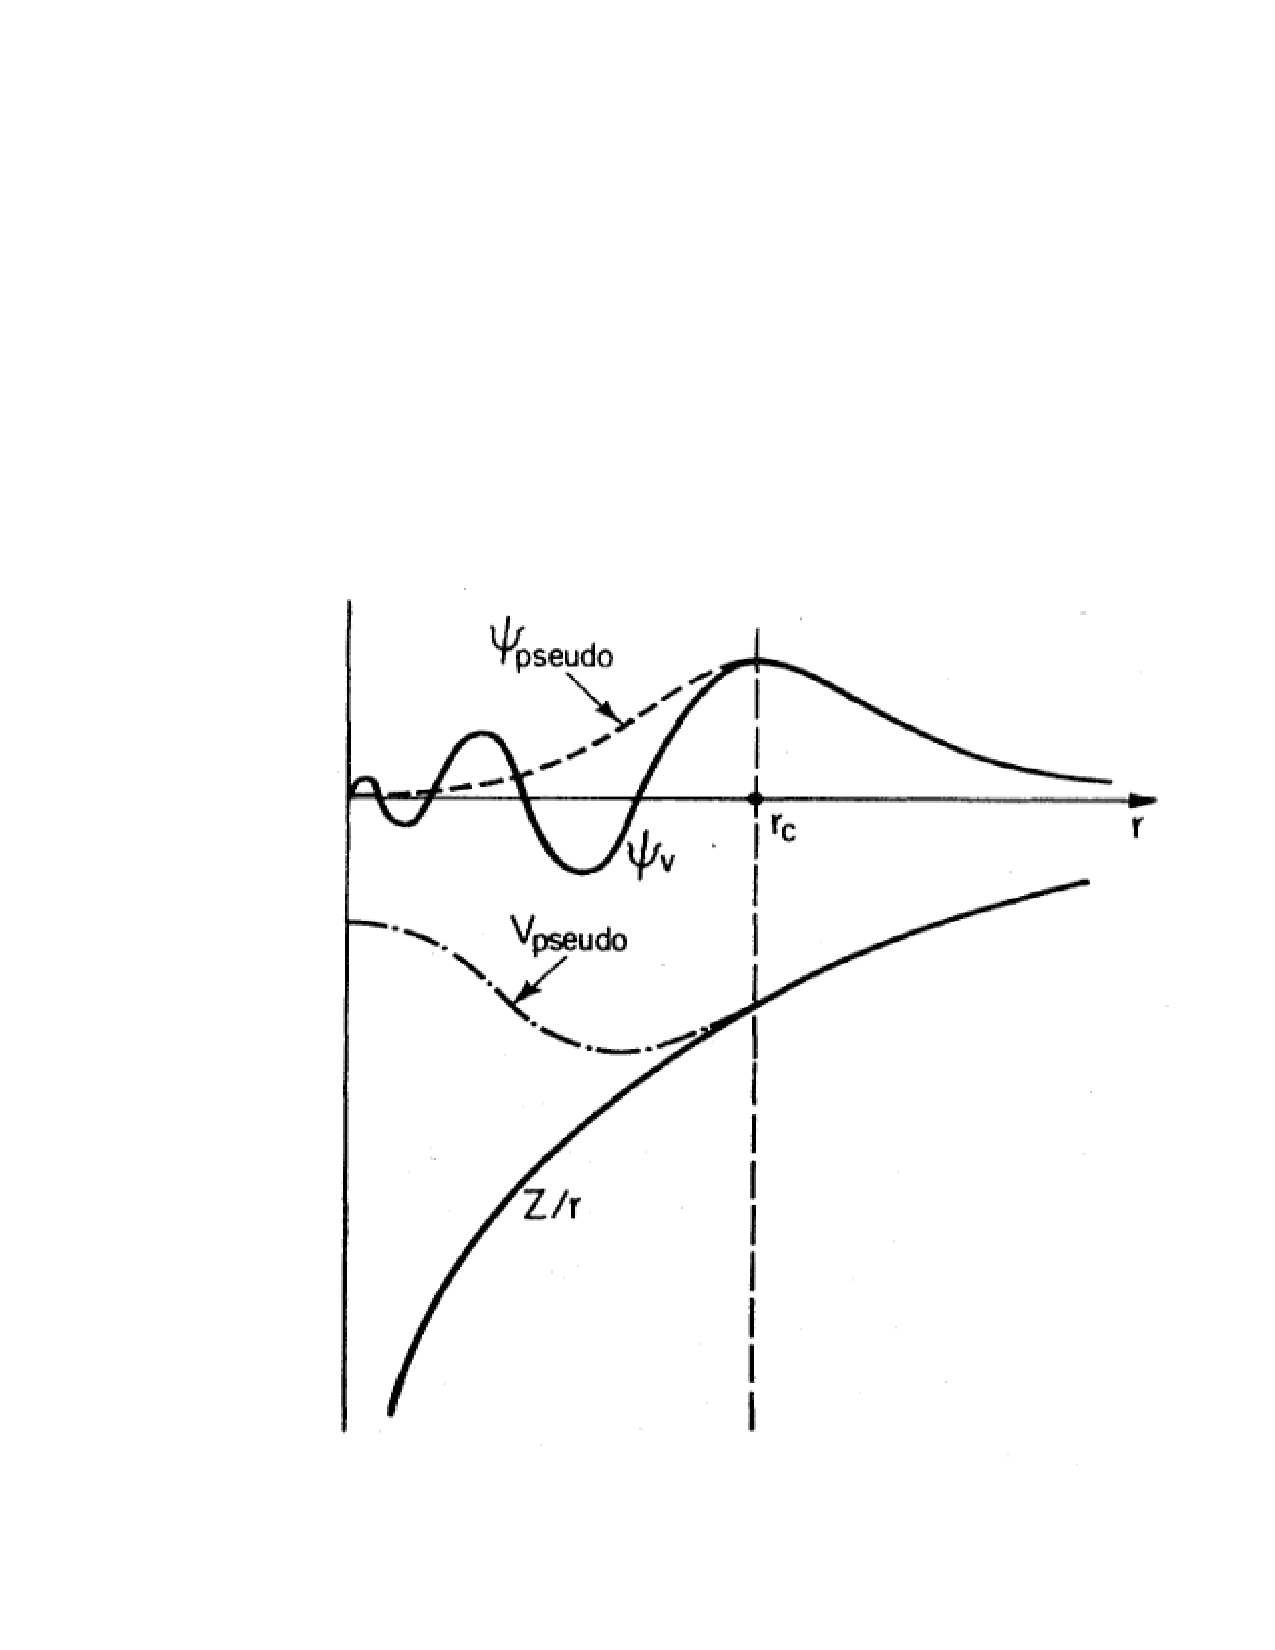
\includegraphics[height=1.35in,width=1.40in,viewport=154 100 562 508,clip]{Figures/Pseudo.pdf}
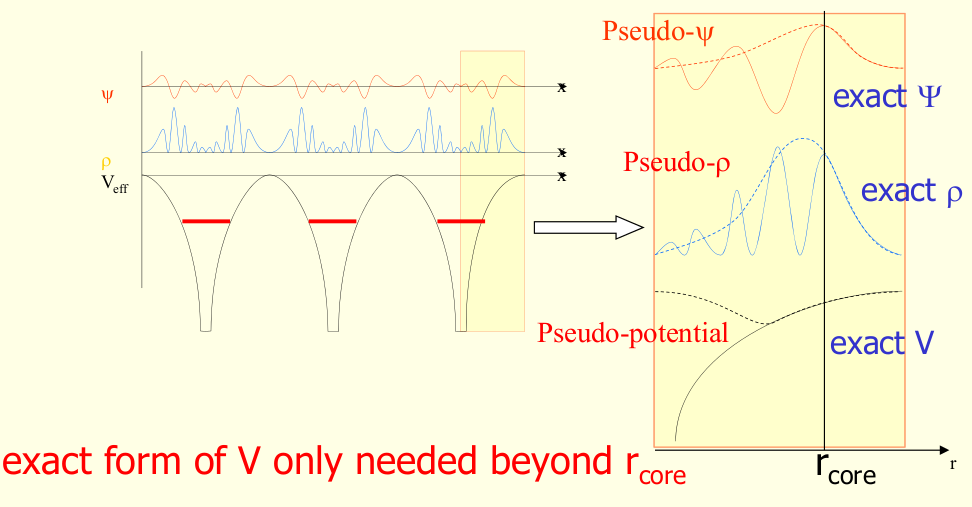
\includegraphics[height=1.35in,width=2.55in,viewport=1 1 980 500,clip]{Figures/Pseudo-2.png}
\caption{\tiny \textrm{The Pseudo wave function and Pseudo potential.}}%(与文献\cite{EPJB33-47_2003}图1对比)
\label{Pseudo_Potential-Wave}
\end{figure}
}

\subsection{模守恒赝势与超软赝势}
\frame
{
	\frametitle{传统赝势的构造}
	直接由实验数据来确定(模型)赝势,常用的实验数据包括离子对电子的散射角度、离子的光谱实验数据等
		\begin{itemize}
			\item 构造离子赝势:~可移植性好
			\item 构造总赝势(包括全部价电子相互作用):~常用于能带描述
		\end{itemize}
%	\begin{itemize}
%		\item 在指定能量范围内,离子对电子散射的散射角
%		\item 离子的光谱实验数据
%	\end{itemize}
\begin{figure}[h!]
\centering
\vspace*{-0.10in}
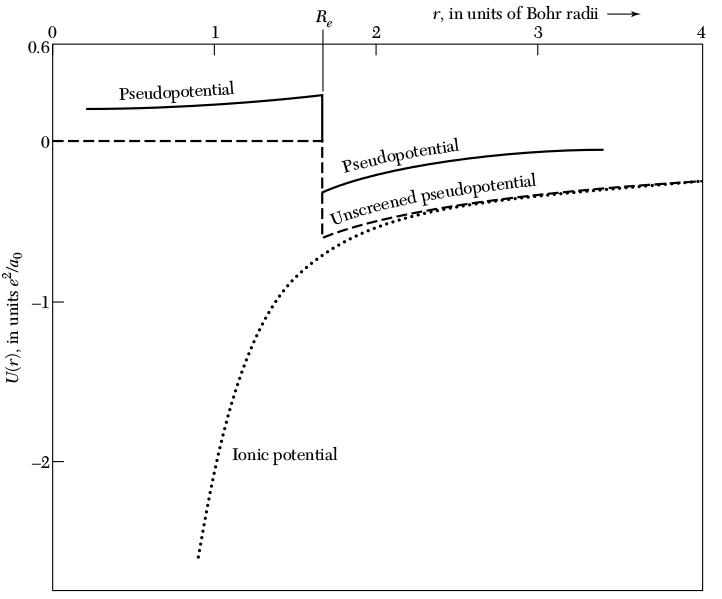
\includegraphics[height=1.60in,width=2.57in,viewport=0 0 980 600,clip]{Figures/Pseudo-model-empty_core.png}
\caption{\tiny \textrm{Pseudopotential for metallic sodium, based on the empty core model and screened by the Thomas-Fermi dielectric function.}}%(与文献\cite{EPJB33-47_2003}图1对比)
\label{Pseudo_model-empty_core}
\end{figure}
}

\frame
{
	\frametitle{传统赝势的构造}
\begin{figure}[h!]
\centering
\vspace*{-0.10in}
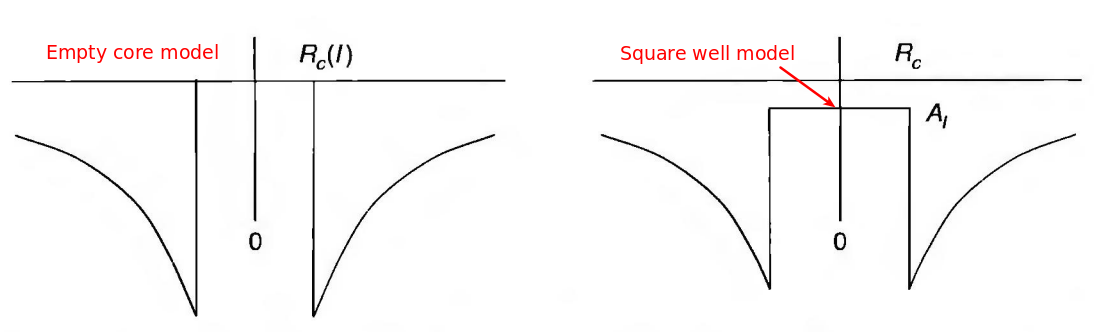
\includegraphics[height=1.30in,width=4.17in,viewport=0 0 1150 350,clip]{Figures/Pseudo-model.png}
\caption{\tiny \textrm{Left:``Empty core'' model potential of Ashcroft in which the potential is zero inside radius $R_c(l)$ which is different for each $l$. Right: Square well model potential with value $A_l$ inside a cut-off radius $R_c$, proposed by Abarenkov and Heine and fit to atomic data by Animalu and Heine. The fact that the potential are weak, zero, or even positive inside cut-off radius $R_c$ is an illustration of the ``cancellation theorem''.}}%(与文献\cite{EPJB33-47_2003}图1对比)
\label{Pseudo-model}
\end{figure}
}

\frame
{
	\frametitle{第一原理赝势}
		由第一原理求解出全电子波函数(径向部分)$P_{n,l}(r)$
			\begin{displaymath}
				\bigg[-\dfrac12\dfrac{\mathrm{d}^2}{\mathrm{d}r^2}+\dfrac{l(l+1)}{2r^2}+V(\rho,r)\bigg]P_{n,l}(r)=\varepsilon_{n,l}P_{n,l}(r)
			\end{displaymath}
			这里$V(\rho,r)$是自洽单电子势
			$$V(\rho,r)=-\frac{Z}r+V_{\mathrm H}(\rho,r)+V_{XC}^{\mathrm{LDA}}(\rho(r))$$
			$V_{\mathrm H}(\rho,r)$是\textrm{Hartree}势,$V_{XC}^{\mathrm{LDA}}(\rho(r))$是交换-相关势

			由此构造赝波函数$P_l^{\mathrm{PP}}(r)$,满足
			$$P_l^{\mathrm{PP}}(r)=P_l^{\mathrm{AE}}(r),\quad r>r_{cl}$$
			进而构造赝势$V_{\mathrm{src},l}^{\mathrm{PP}}(r)$
			$$V_{\mathrm{src},l}^{\mathrm{PP}}(r)=\varepsilon_l-\dfrac{l(l+2)}{2r^2}+\dfrac{1}{2P_l^{\mathrm{PP}}(r)}\dfrac{\mathrm{d}^2}{\mathrm{d}r^2}P_l^{\mathrm{AE}}(r),\quad r>r_{cl}$$
}

\frame
{
	\frametitle{模守恒\textrm{(Norm-conserving)}条件}
%	构造赝势确定参数的边界(构造条件)
	\begin{enumerate}
		\item 价电子赝波函数的能量本征值与对应全电子波函数能量本征值相等:~$\varepsilon_l^{\mathrm{PP}}=\varepsilon_l^{\mathrm{AE}}$
		\item 价电子赝波函数与真实电子波函数的径向部分在截断半径$r_{c,l}$外相同:~$\psi_l^{\mathrm{PP}}(r)=\psi_l^{\mathrm{AE}}(r),\quad r>r_{cl}$
		\item 价电子赝波函数与真实电子波函数的对数导数在截断半径$r_{c,l}$处相等:~$D_l^{\mathrm{PP}}(r)=D_l^{\mathrm{AE}}(r),\quad r\geqslant r_{cl}$\\
		这里$D_l(\varepsilon,r)=r\frac{\psi_l^{\prime}(\varepsilon,r)}{\psi_l(\varepsilon,r)}=r\dfrac{\mathrm{d}}{\mathrm{d}r}\ln\psi_l(\varepsilon,r)$
		\item 价电子赝波函数与真实电子波函数在截断半径$r_{c,l}$内的积分电荷相等(\textcolor{red}{模守恒条件})
			$$Q_l=\int_0^{r_{cl}}\mathrm{d}rr^2|\psi_l^{\mathrm{PP}}(r)|^2=\int_0^{r_{cl}}\mathrm{d}rr^2|\psi_l^{\mathrm{AE}}(r)|^2$$
		\item 价电子赝波函数与真实电子波函数的对数导数一阶能量导数$\mathrm{d}D_l(\varepsilon,r)/\mathrm{d}\varepsilon$在截断半径$r_{c,l}$处及以外相等
	\end{enumerate}
}

\frame
{
	\frametitle{模守恒\textrm{(Norm-conserving)}条件}
\begin{figure}[h!]
\centering
\vspace*{-0.10in}
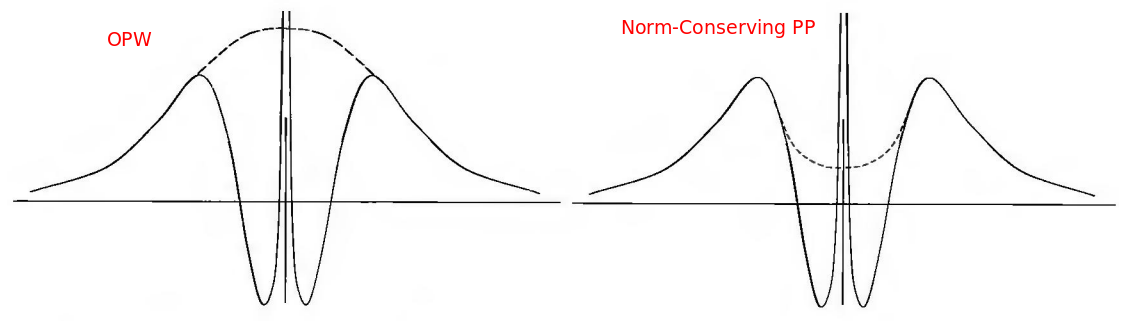
\includegraphics[height=1.30in,width=4.17in,viewport=0 0 1150 350,clip]{Figures/Pseudo-OPW_NCPP.png}
\caption{\tiny \textrm{Schematic example of a valence function that has the character of a $3s$ orbital near the nucleus and two examples of smooth functions (dashed lines) that equal the full wave-function outside the core region. Left: the smooth part of the valence function defined by OPW-like equation; Right: a smooth pseudo-function that satisfies the norm-conservation condition.}}%(与文献\cite{EPJB33-47_2003}图1对比)
\label{Pseudo-OPW_NCPP}
\end{figure}
}

\frame
{
	\frametitle{赝势去屏蔽与非局域化}
	第一原理赝势建立了赝波函数与对应赝势的一一对应关系,但该赝势包含了电子屏蔽(原子、离子环境)信息,去屏蔽后的赝势对环境依赖更低,“可移植性”更好
	$$V_{\mathrm{ion},l}^{\mathrm{PP}}(r)=V_{\mathrm{src},l}^{\mathrm{PP}}(r)-V_{\mathrm{H},l}^{\mathrm{PP}}(r)-V_{XC,l}^{\mathrm{PP}}(r)$$
	去屏蔽过程中,特别需要注意$V_{XC,l}^{\mathrm{PP}}(r)$的处理
	$$V_{XC}^{\mathrm{PP}}(r)=V_{XC}^{\mathrm{PP}}([n^{\mathrm{PP}}],r)+\big[V_{XC,l}^{\mathrm{PP}}([n^{\mathrm{PP}}+n^{core}],r)-V_{XC}^{\mathrm{PP}}([n^{\mathrm{PP}}],r)\big]$$
	{\fontsize{7.2pt}{5.2pt}\selectfont{如果定义辅助函数}}
	$$\chi_{lm}^{\mathrm{PP}}(\vec r)=\bigg\{\varepsilon_l-\bigg[-\dfrac12\nabla^2+V_{\mathrm{local}}^{\mathrm{PP}}(\vec r)\bigg]\bigg\}\psi_{lm}^{\mathrm{PP}}(\vec r)$$
	{\fontsize{7.2pt}{5.2pt}\selectfont{赝势可以分解为局域部分与非局域部分之和称为可分离赝势(也称\textrm{factroided pseudo-potential})}}
	$$V_{NL}^{\mathrm{PP}}(r)=V_{\mathrm{local}}^{\mathrm{PP}}(r)+\sum_{lm}\dfrac{|\chi_{lm}^{\mathrm{PP}}\rangle\langle\chi_{lm}^{\mathrm{PP}}|}{\langle\chi_{lm}^{\mathrm{PP}}|\psi_{lm}^{\mathrm{PP}}\rangle}=V_{\mathrm{local}}^{\mathrm{PP}}(r)+\sum_{lm}\dfrac{|\psi_{lm}^{\mathrm{PP}}\delta V_l\rangle\langle\delta V_l\psi_{lm}^{\mathrm{PP}}|}{\langle\psi_{lm}^{\mathrm{PP}}|\delta V_l|\psi_{lm}^{\mathrm{PP}}\rangle}$$
}

\frame
{
	\frametitle{模守恒赝势构造流程}
\begin{figure}[h!]
\centering
%\vspace*{-0.10in}
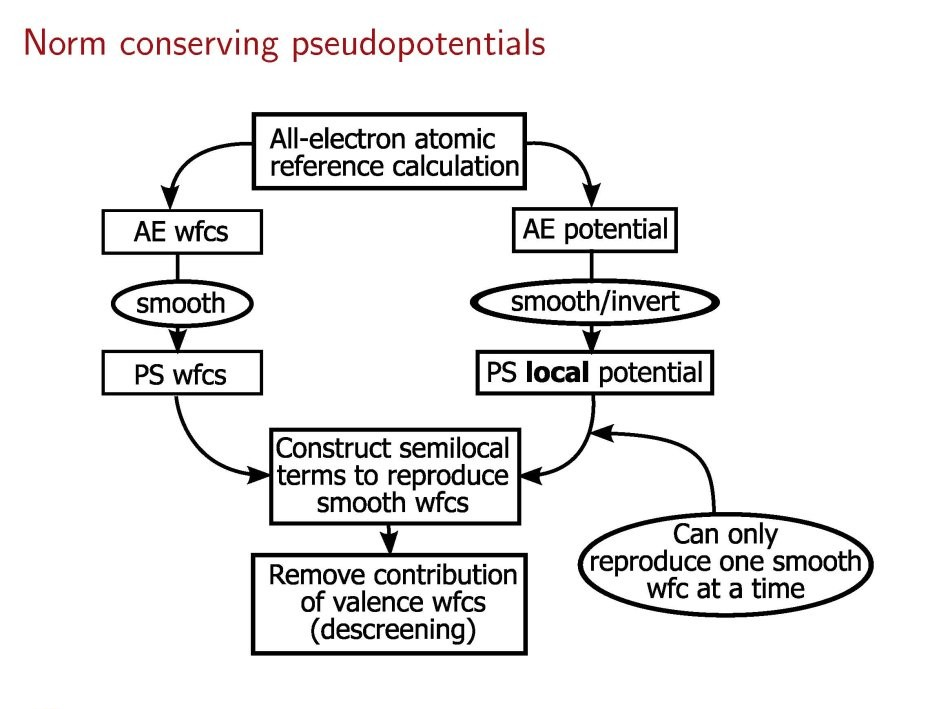
\includegraphics[height=2.70in,width=3.77in,viewport=70 40 900 610,clip]{Figures/Pseudo-NC.jpg}
%\caption{\tiny \textrm{Pseudopotential for metallic sodium, based on the empty core model and screened by the Thomas-Fermi dielectric function.}}%(与文献\cite{EPJB33-47_2003}图1对比)
\label{Pseudo-NC}
\end{figure}
}

